\documentclass{article}

\usepackage{hyperref} %for hyperlinking
\usepackage{libertine} %fancy font
\usepackage{graphicx} %for images
\setkeys{Gin}{width=1\textwidth} %sets default width for graphics
\usepackage{listings} %for code chunks
\usepackage[british]{babel} %to get the right hyphenation rules
\usepackage{amsmath} %for multi-line equations
%\usepackage{doi} %for doi conversion to hyperlinks
%\usepackage{caption} %for subplots
%\usepackage{subcaption} %for subplots

\title{Computational Study}
\author{}
\date{} 

\begin{document}
\maketitle
%\sloppy

\section{Introduction}

I am interested in the question of whether a melanopic signal might be useful to estimate the illuminant(s) in a scene.

Following initial psychophysical experiments, where results did not indicate a strong or simple relationship, I chose to take a step back and examine the problem that the HVS is faced with in a natural environment, which colour constancy solves. Through this route I hoped to answer the questions:
\begin{enumerate}
	\item Would it be sensible for the HVS to use a melanopic signal to help solve this problem?
	\item If so, in what way would it be used?
\end{enumerate}

In this document I shall give an overview of the main scripts I have written, going through the logic and results of each.
All scripts are available at \url{https://github.com/da5nsy/Melanopsin_Computational}

\section{melcomp\_1}

In melcomp\_1 I set out with three questions:
\begin{enumerate}
\item Considering only daylight spectra (excluding reflective surfaces for now), can a melanopic signal predict the chromaticity of daylight more precisely than signals provided by other retinal cell populations?
\item Now considering also object reflectances, does a melanopic signal provide a means of calculating a sign and weight of shift required to counteract the chromatic shift induced upon objects by a change in daylight conditions?
\item Are there objects, or luminance levels, or daylight chromaticities for which the melanopic signal is particularly effective or ineffective at performing the above task
\end{enumerate}

The final question was asked with the hope that such limitations might provide nice tests to perform psychophysically. 

Foundational data consisting of the Granada daylight dataset, the Stockman-Sharpe 10 degree cone fundamentals, the Lucas et al. melanopsin fundamental, and the a subset of the Vrhel et al. reflectances (consisting of the `natural' reflectances) were used.

Tristimulus values $[L,M,S]$ and analogous melanopic values ($I$) were calculated for each illuminant within the Granada dataset. The real-world correlate of this computation would be to observe a spectralon tile under each daylight condition.

MacLeod-Boynton chromaticity co-ordinates were calculated, and three-dimensional plots were made to display $l_{\text{MB}}$ against $s_{\text{MB}}$ against $[L,M,S,I]$ in turn. Each plot is shown in \ref{fig:l1}. As can be seen, although there exists some relationship between the chromaticity values and the first level values, it does not appear as though one could predict the other. All that can be said from this relationship is that if the first level value is above a certain threshold, it is likely to be in a group with a low $s_{\text{MB}}$ value. The real-world correlate of this is to say - \textit{if the day is bright enough, I can be fairly confident that the chromaticity of daylight will be relatively warm in colour.} This is as expected, since the brightest daylight conditions are likely to be those with unobstructed direct sunlight, which is warmer in colour than illumination provided by the blue sky. This relationship seems relatively weak however, and could not be used to accurately predict the chromaticity of an illuminant. The answer to the first question set out for the script then, is that a melanopic signal cannot predict chromaticity (though neither can any other signal).

\begin{figure}[ht]
    \centering
    \includegraphics{C:/Users/cege-user/Dropbox/Documents/MATLAB/Melanopsin_Computational/figs/melcomp_1/level1sigspredictingColorimetry.pdf}
    \caption{Caption}
    \label{fig:l1}
\end{figure} 

\begin{figure}[ht]
    \centering
    \includegraphics{C:/Users/cege-user/Dropbox/Documents/MATLAB/Melanopsin_Computational/figs/melcomp_1/correlationBetweenLevel1Sigs.pdf}
    \caption{The relationship between melanopic power (analogous to a tristimulus value but calculated using the spectral sensitivity of melanopsin) with the traditional tristimulus values showing a strong correlation. Red points indicate signals computed directly from the spectral power distribution, grey points represent values of computed colorimetry for objects under illuminants.}
    \label{fig:tristimCorrelation}
\end{figure} 

It should be noted that there was very high correlation between each signal. This can be considered as corresponding to the high importance of the first principal component of the spectral measurements in this dataset. Put another way, a sensor with almost any spectral sensitivity could be used to estimate the magnitude of the daylight. I shall return to the discussion of principal components when discussing melcomp\_3.

\begin{minipage}{\linewidth}
\begin{lstlisting}
corr(LMSM')

    1.0000    1.0000    0.9993    0.9998
    1.0000    1.0000    0.9995    0.9999
    0.9993    0.9995    1.0000    0.9999
    0.9998    0.9999    0.9999    1.0000
\end{lstlisting}
\end{minipage}

Following this, similar plots were made which plotted $l_{\text{MB}}$ against $s_{\text{MB}}$ as before, but now plotted the various combinations of $[L,M,S,I]$ created by considering one signal over another (e.g. $L/M$). Following the terminology of \cite{barrionuevo_contributions_2014} I shall refer to $[L,M,S,I]$ as `first level signals' and these derived signals as `second level signals'. The twelve plots created all showed clear and relatively simple relationships between chromaticity and these new derived signals.

For many of these signals however, such relationships are to be expected. For example, a relationship between $l_{\text{MB}}$ and $L/M$ should be expected, since $l_{\text{MB}}$ is defined as the sum of weighted components of $L$ and $M$. To confirm this, a null condition was performed, where $[L,M,S,I]$ was replaced by randomly generated values, and the second level signals were generated as before. Relationships between secondary signals derived from L, M or S signals still showed correlations with chromaticity (albeit now points fell on a plane, instead of a line), whereas signals with a $I$ component showed only minimal coherence, forming a rough cloud in three-dimensional space. 

This example shows that a melanopic signal exhibits correlation with a chromatic signal \emph{not} due to the underlying mathematics of how chromaticity is calculated, and that any relationship must follow from a genuine regularity in the data.

Following this, reflectances were introduced, so as to consider a slightly more realistic situation. Now the simulation considered the colour signals produced by each of the recorded reflectances, under each of the recorded illuminants. MacLeod-Boynton chromaticities, and an analogous melanopic signal, were computed as defined by equation \ref{eq:i} (see \cite{macleod_chromaticity_1979} and \cite{cie_cie_2015}), where $k_1$ and $k_2$ represent the constants required such that the sum of the weighted $L$ and $M$ signals equals or approximates the luminance function. Chromaticities are plotted in figure \ref{fig:mb}.

\begin{equation} \label{eq:i}
i_{MB} = I/(k_1L + k_2M) 
\end{equation}

\begin{figure}[ht]
    \centering
    \includegraphics{C:/Users/cege-user/Dropbox/Documents/MATLAB/Melanopsin_Computational/figs/melcomp_1/BasicMB.pdf}
    \caption{$l_{\text{MB}}$ (MB1 above) against $s_{\text{MB}}$ (MB2 above). MacLeod-Boynton chromaticities for 12 reflectances under 2600 daylight illuminants.}
    \label{fig:mb}
\end{figure} 

Now able to consider the second question, I considered whether it was possible to perform a conversion of these computed chromaticities into a hypothetical illuminant-independent space, using $i_{\text{MB}}$ as a corrective signal. It was found through an optimization procedure that through addition and subtraction of weighted $i_{\text{MB}}$ values, using the scaling factors shown in equation \ref{eq:correction} such a conversion could approximately be performed. The results of applying equation \ref{eq:correction} can be seen in figure \ref{fig:corrected}.

\begin{subequations} \label{eq:correction}
%\begin{align}
$l_{\text{MB}}$* = $l_{\text{MB}}$ + 0.23$i_{\text{MB}}$\\
$s_{\text{MB}}$* = $s_{\text{MB}}$ - 1.70$i_{\text{MB}}$
%\end{align}
\end{subequations}

\begin{figure}[ht]
    \centering
    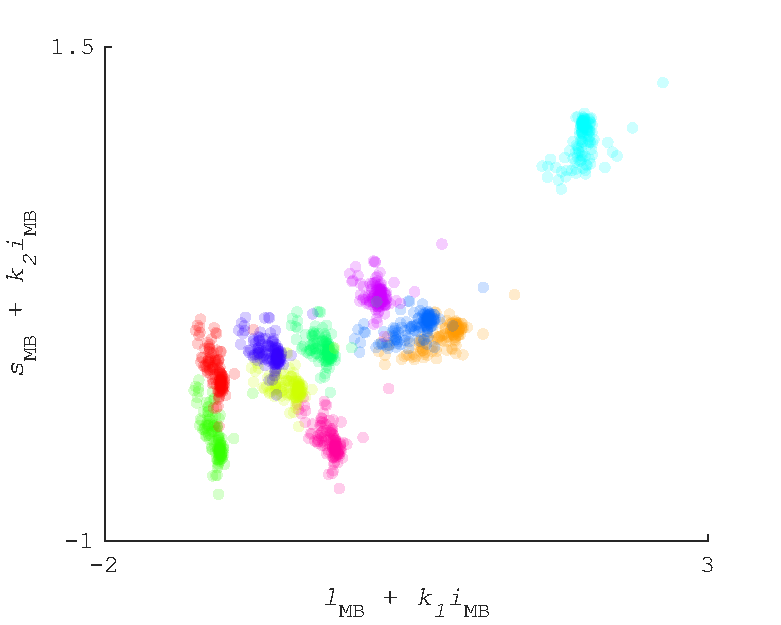
\includegraphics{C:/Users/cege-user/Dropbox/Documents/MATLAB/Melanopsin_Computational/figs/melcomp_1/correctedChromaticities.pdf}
    \caption{$l_{\text{MB}}$* (MBx1 above) against $s_{\text{MB}}$* (MBx2 above). MacLeod-Boynton chromaticities for 12 reflectances under 2600 daylight illuminants, corrected by the corresponding $i_{\text{MB}}$ value.}
    \label{fig:corrected}
\end{figure} 

It can be seen that the points are no longer smeared by the impact of illumination, and instead roughly cluster together by object.

Following this, an additional optimization procedure was performed, to consider whether shifting the sensitivity of the melanopsin function along the wavelength spectrum affected the performance of such a signal in correcting these values. The optimization sought to minimise the overall spread of chromaticities (measured as standard deviation of the entire set). The results of this optimisation can be seen in figure \ref{fig:opt}. It can be seen that minima for $l_{\text{MB}}$* occur at around 530nm and just under 600nm, and minima for $s_{\text{MB}}$* occur at around 450nm and 580nm. On first appearance this seems to suggest that the optimal spectral sensitivity for a cone type employed to correct the signals from the various cones might be around these points in the spectrum. However, the careful reader might note the correspondence between the figures above and the peak spectral sensitivities of the cones themselves (S-448nm, M-541nm, L-569nm). Indeed we see that the optimal performance occurs when the nominal melanopsin sensitivity overlaps most well with the spectral sensitivity of the cones. It is understandable why this occurs - each signal is then normalised by a near-duplicate of itself, rendering each value in the set being close to zero.

\begin{figure}[ht]
    \centering
    \includegraphics{C:/Users/cege-user/Dropbox/Documents/MATLAB/Melanopsin_Computational/figs/melcomp_1/minimiseSD.pdf}
    \caption{caption}
    \label{fig:opt}
\end{figure} 

\begin{figure}[ht]
    \centering
    \includegraphics{C:/Users/cege-user/Dropbox/Documents/MATLAB/Melanopsin_Computational/figs/melcomp_1_caller/opt.pdf}
    \caption{The results of an optimization where the spectral sensitivity of the nominal melanopsin fundamental was shifted along the spectrum. Generated using melcomp\_1\_caller.m for iteration.}
    \label{fig:opt}
\end{figure} 

This had the unexpected and unfortunate effect of simply crushing all the chromaticties down onto a single line, without preserving any inter-object chromatic differences. We witness perfect colour constancy, at the expense of any chromatic discrimination. This is obviously not ideal.

\begin{figure}[ht]
    \centering
    \includegraphics{C:/Users/cege-user/Dropbox/Documents/MATLAB/Melanopsin_Computational/figs/melcomp_1_caller/sdmeans.pdf}
    \caption{Normalised average distance between points in the set of the mean chromaticities for the different reflectances. It can be seen that inter-reflectance variation drops to zero at the same minima as seen in figure \ref{fig:opt}, showing that these distinct points are undesirably corrected to the same point. Generated using melcomp\_1\_caller.m for iteration.}
    \label{fig:sdmeans}
\end{figure} 

The work was presented at this stage as a poster at VSS in 2018, which is available at \url{doi.org/10.6084/m9.figshare.6280865}.

The actual desired behaviour would be to minimise internal variance for each reflectance group, whilst maintaining at least some distinction between inter-reflectance groups. A more comprehensive approach to this question would need to consider the relative importance of the two separate requirements, and apply appropriate weightings.

\bibliographystyle{alpha}
\bibliography{MyLibrary}

\end{document}

%\begin{figure}
%     \centering
%     \begin{subfigure}[b]{0.49\textwidth}
%         \centering
%         \includegraphics[width=\textwidth]{figs/mb.pdf}
%         \caption{$y=x$}
%         \label{fig:y equals x}
%     \end{subfigure}
%     \hfill
%     \begin{subfigure}[b]{0.49\textwidth}
%         \centering
%         \includegraphics[width=\textwidth]{figs/corrected.pdf}
%         \caption{$y=3sinx$}
%         \label{fig:three sin x}
%     \end{subfigure}
%     \hfill
%        \caption{Three simple graphs}
%        \label{fig:three graphs}
%\end{figure}
